\documentclass[tikz,border=10pt]{standalone}
\usepackage{pgfplots}
\usetikzlibrary{intersections, calc}

\begin{document}
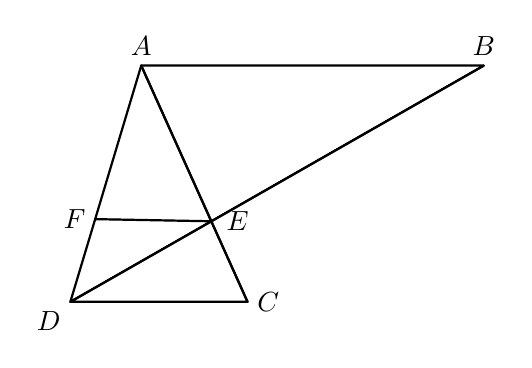
\begin{tikzpicture}[line join=round, line cap=round, >=stealth, scale=1.5]
    % --- 1. 定义关键顶点坐标 ---
    % 设定基准点 D 为原点，C 在 x 轴上
    \coordinate (D) at (0,0);
    \coordinate (C) at (1.5, 0);
    \coordinate (A) at (0.6, 2);
    \coordinate (B) at (3.5, 2); % AB 保持平行于 CD (y值相同)

    % --- 2. 计算交点 E ---
    % E 是 AC 和 BD 的交点
    \path [name path=lineAC] (A) -- (C);
    \path [name path=lineBD] (B) -- (D);
    \path [name intersections={of=lineAC and lineBD, by=E}];

    % --- 3. 计算点 F ---
    % F 在 AD 上，且 EF 平行于 CD (即 y坐标与 E 相同)
    % 获取 E 的 y 坐标

    \path [name path=horizE] (0, 0.7) -- (2, 0.7);
    \path [name path=lineAD] (A) -- (D);
    \path [name intersections={of=horizE and lineAD, by=F}];
\draw(E)--(F);
    % --- 4. 绘制图形轮廓 ---
    \draw [thick] (A) -- (B) -- (D) -- (C) -- cycle; % 绘制四边形轨迹
    \draw [thick] (A) -- (C);        % 对角线 AC
    \draw [thick] (B) -- (D);        % 对角线 BD
    \draw [thick] (F) -- (E);        % 线段 EF
\draw [thick] (A) -- (D);
    % --- 5. 标注点名称 ---
    % 使用 pos 控制文字距离，便于微调
    \node [above] at (A) {$A$};
    \node [above] at (B) {$B$};
    \node [right] at (C) {$C$};
    \node [below left] at (D) {$D$};
    \node [right, xshift=2pt] at (E) {$E$};
    \node [left]  at (F) {$F$};

\end{tikzpicture}
\end{document}